\documentclass[english,serif,mathserif]{beamer}
\usetheme[formal,deutsch]{s3it}

\usepackage{graphicx}
\usepackage[T1]{fontenc}
\usepackage[latin9]{inputenc}
\usepackage{babel}
\usepackage{color}

\begin{document}

%% Optional Argument in [Brackets]: Short Title for Footline
\title[Short Title]{MySQL and RabbitMQ} 
\subtitle{Or: OpenStack's core support softwares} 

\author{Tyanko Aleksiev \texttt{<tyanko.aleksiev@s3it.uzh.ch>}}

\date{\today}

\maketitle

% chapter division
\begin{frame}{MySQL's role inside OpenStack}

\textit{MySQL} database assumes a core role in the set of support softwares
inside OpenStack and is mainly used:

\begin{itemize}
\item for storing the state of the OpenStack cluster (VMs, users, volumes, tokens, etc), 
\item in the workflow of handling the various service requests (e.g. starting a new instance, creating a volume).
\end{itemize}

An alternative of MySQL in OpenStack could be any database supported by sqlalchemy.

\end{frame}

\begin{frame}{RabbitMQ's role inside OpenStack}

The \textit{RabbitMQ} messaging system, used like Remote Procedure Call (RPC),
is the second core support software and is mainly used:

\begin{itemize}
\item to provide a communication layer between the different stack components, 
\item as a consequence to enable the collaboration between the components.
\end{itemize} 

The usage of RabbitMQ prevents the processes from polling the DB at every interaction. 

\vspace{5mm}

Alternatives of RabbitMQ inside OpenStack are Qpid and ZeroMQ.

\end{frame}
\begin{frame}{Example of RabbitMQ and MySQL usage during instance creation}

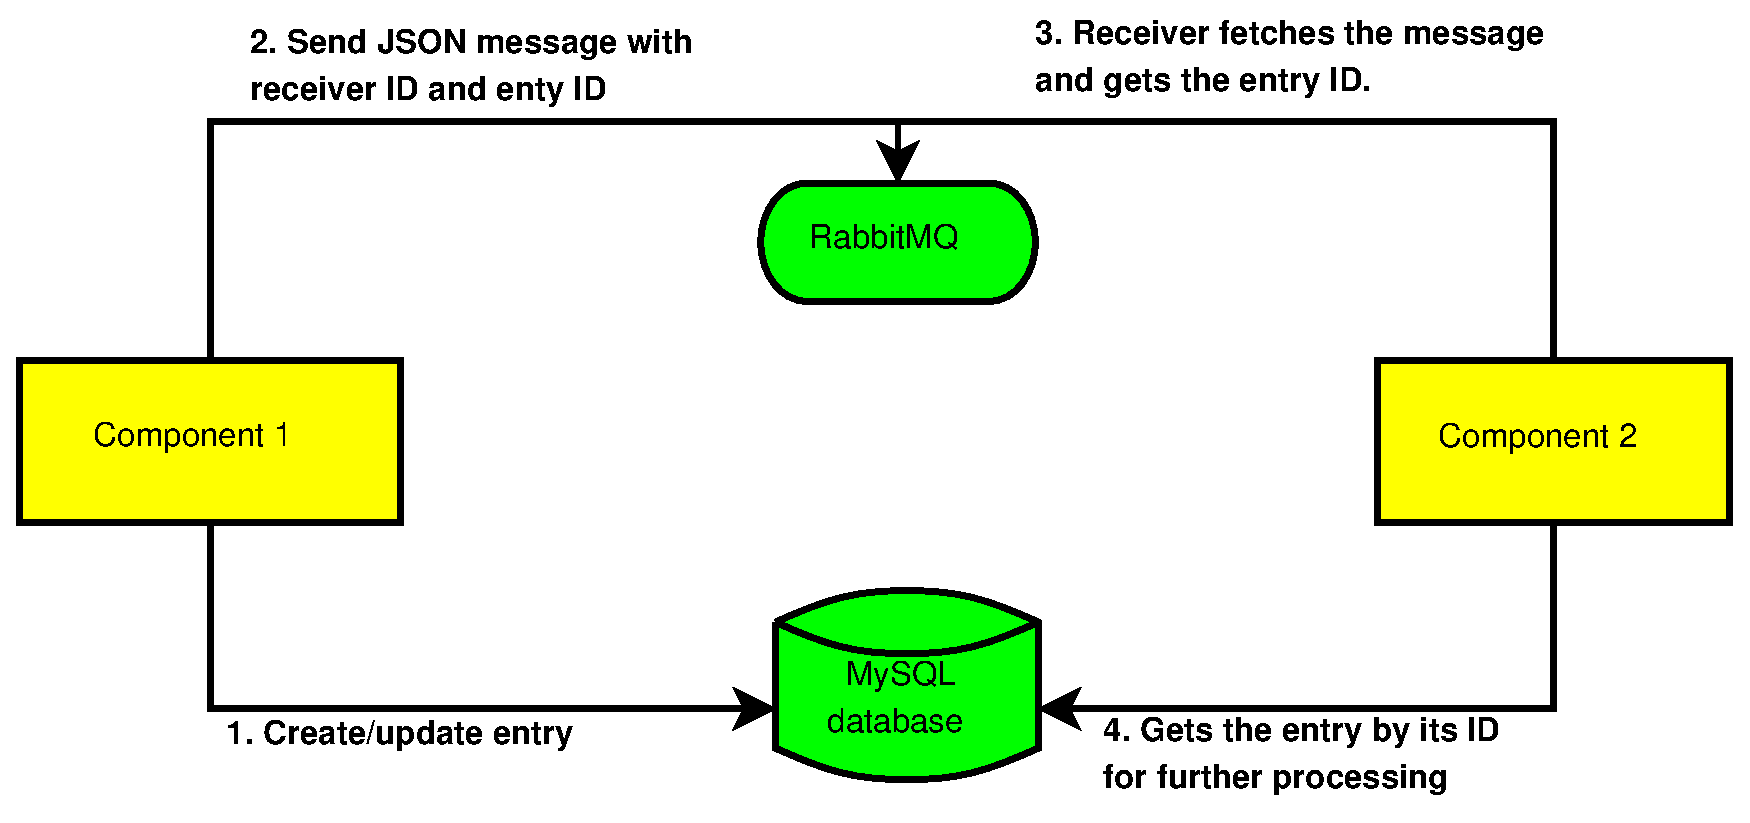
\includegraphics[scale=0.37]{db-rabbitmq.eps}

\end{frame}
\begin{frame}{Example of RabbitMQ and MySQL usage during instance creation}

\begin{itemize}
\item a client sends a POST request to nova-api for a VM provisioning,
\item nova-api writes an entry in the \textbf{DB},
\item nova-api posts then a JSON message in \textbf{RabbitMQ} queue (the message is for nova-scheduler),
\item nova-scheduler reads the JSON message from \textbf{RabbitMQ},
\item it examines the overall cluster situation from the \textbf{DB},
\item nova-scheduler then decides which compute should start the VM and posts JSON message in its \textbf{RabbitMQ} queue,
\item nova-compute gathers then the request information (from the \textbf{RabbitMQ} and \textbf{DB}) and proceeds with the VM provisioning.
\end{itemize}

\end{frame}

\begin{frame}{MySQL High Availabiltiy}

MySQL is one of the most critical components because it contains
the state of the whole Stack.

\vspace{5 mm}

Having MySQL in HA becomes almost a requirement. OpenStack's recommended way to 
do it is by using the master - slave replication implementing DRBD and Pacemaker.

\vspace{5mm}

An active - active (N+1) alternative is using a Galera cluster which should become the 
state-of-the-art in the near future. 

\vspace{5 mm}

{\color{blue}\href{http://docs.openstack.org/high-availability-guide/content/s-mysql.html}{This}} 
link provides more information.

\end{frame}

\begin{frame}{RabbitMQ High Availabiltiy}

RabbitMQ can be configured in HA to prevent communication failure between the OpenStack components.

\vspace{5 mm}

This can be achieved again, like in the case with MySQL, by using DRBD and Pacemaker. 

\vspace{5mm}

An alternative method, by using again active - active 
(even if implementation is actually active - salve) mirrored servers. 

\vspace{5 mm}

{\color{blue}\href{http://docs.openstack.org/high-availability-guide/content/s-rabbitmq.html}{This}} 
link provides detailed information. 

\end{frame}

\begin{frame}{Notes and Remarks}

\begin{itemize}
\item Installation of MySQL and RabbitMQ is really straight forward
and requires limited intervention. 
\item Configuration of RabbitMQ is limited to changing the default passwd and the bind address.
      \begin{itemize}
          \item Conf. file is \texttt{/etc/rabbitmq/rabbitmq-env.conf}
          \item Logs directory is: \texttt{/var/log/rabbitmq} 
      \end{itemize} 
\item Configuration of MySQL requires a little bit more than RabbitMQ.
      \begin{itemize}
        \item Conf. file is: \texttt{/etc/mysql/my.cnf}
        \item Logs directory is: \texttt{/var/log/mysql}
      \end{itemize}
\item We will see everything in more detail during the tutorial.
\end{itemize}

\end{frame}

\end{document}

%%% Local Variables:
%%% mode: latex
%%% TeX-master: t
%%% End:
